\documentclass[10pt]{beamer}

% ------------------------------------------------------------------------
% Carga del preámbulo personalizado (preamble.tex)
% (Asegúrate de tenerlo en la misma carpeta para que \input funcione)
% ------------------------------------------------------------------------
\usetheme[progressbar=frametitle]{metropolis}
\usepackage{appendixnumberbeamer}
\usepackage{fancyvrb}
\usepackage{booktabs}
\usepackage[scale=2]{ccicons}
\usepackage{pgfplots}
\usepgfplotslibrary{dateplot}
\usepackage{type1cm}
\usepackage{lettrine}
\usepackage{ragged2e}
\usepackage{xspace}
\newcommand{\themename}{\textbf{\textsc{metropolis}}\xspace}
\usepackage{graphicx} % Allows including images
\usepackage{booktabs} % Allows the use of \toprule, \midrule and \bottomrule in tables
\usepackage[utf8]{inputenc} %solucion del problema de los acentos.
\usepackage{xcolor}
\definecolor{LightGray}{gray}{0.9}

\usepackage{minted}
\usemintedstyle{tango}
\newcommand{\mypyfile}[1]{\inputminted[linenos=true, fontsize=\footnotesize, frame=lines, framesep=5\fboxrule,framerule=1pt]{python}{#1}}

\setminted[python]{breaklines,frame=lines,framesep=2mm,baselinestretch=1.2,bgcolor=LightGray,linenos, fontsize=\footnotesize} % obeytabs=true, tabsize=2, showtabs=true}

%%%%%%%%%%%%%%%%%%%%%%%%%%%%%%%%%%%%%%%%%%%%%%%%%%%%%%%%%%%%%%%%%%%%%%%%%%%%%%%%%%%%%%
\setbeamercolor{progress bar}{fg=blue!50!black,bg=white!50!black}
\setbeamercolor{title separator}{fg=red!50!black,bg=white!50!black}
\setbeamercolor{frametitle}{fg=white!80!black,bg=red!50!black}
\title[PCFI161]{Programaci\'on para F\'isica y Astronom\'ia}
\subtitle{Departamento de Física.}

\newcommand{\myfront}{
\author[PCFI161]{Corodinadora: C Loyola \\ Profesoras/es C Loyola / C Femenías / Y Navarrete / C Ruiz}
\institute[UNAB]{Universidad Andrés Bello}
\date{Primer Semestre 2025}
}

\titlegraphic{%
  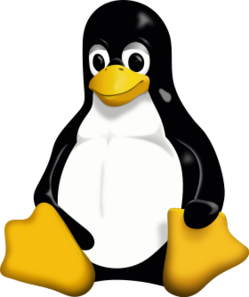
\includegraphics[width=.08\textwidth]{logo-tux.png}\hfill
  
\includegraphics[width=.3\textwidth]{logo-unab.png}\hfill
  
\includegraphics[width=.08\textwidth]{logo-python.png}
}

\makeatletter
\setbeamertemplate{title page}{
  \begin{minipage}[b][\paperheight]{\textwidth}
    \vfill%
    \ifx\inserttitle\@empty\else\usebeamertemplate*{title}\fi
    \ifx\insertsubtitle\@empty\else\usebeamertemplate*{subtitle}\fi
    \usebeamertemplate*{title separator}
    \ifx\beamer@shortauthor\@empty\else\usebeamertemplate*{author}\fi
    \ifx\insertdate\@empty\else\usebeamertemplate*{date}\fi
    \ifx\insertinstitute\@empty\else\usebeamertemplate*{institute}\fi
    \vfill
    \ifx\inserttitlegraphic\@empty\else\inserttitlegraphic\fi
    \vspace*{1cm}
  \end{minipage}
}
\makeatother


\makeatletter
\setlength{\metropolis@titleseparator@linewidth}{2pt}
\setlength{\metropolis@progressonsectionpage@linewidth}{2pt}
\setlength{\metropolis@progressinheadfoot@linewidth}{2pt}
\makeatother


\begin{document}

% ------------------------------------------------------------------------
% Portada de la Presentación
% ------------------------------------------------------------------------
\myfront{}

% ------------------------------------------------------------------------
% Slide 1: Título de la Sesión
% ------------------------------------------------------------------------
\begin{frame}[plain]
  \titlepage
  % Título de la sesión: Ejercicios Organizados por Estructuras de Control
\end{frame}

% ------------------------------------------------------------------------
% Slide 2: Índice / Tabla de Contenidos
% ------------------------------------------------------------------------
\begin{frame}
  \frametitle{Ejercicios Organizados por Estructuras de Control}
  \tableofcontents
\end{frame}

% ------------------------------------------------------------------------
% Configuración de bloques (en caso de usar metrópolis u otro tema)
% ------------------------------------------------------------------------
\metroset{block=fill}

% ----------------------------------------------------------------------------------------
% SECCIÓN 1: Introducción
% ----------------------------------------------------------------------------------------
\section{Introducción}

% ------------------------------------------------------------------------
% Slide 3: Criterios de Organización
% ------------------------------------------------------------------------
\begin{frame}{Criterios de Organización}
  \begin{itemize}
    \item \textbf{Separación por estructura de control}:
      \begin{itemize}
        \item Ejercicios con \texttt{if-elif-else} (condicionales)
        \item Ejercicios con \texttt{for/while} (bucles)
        \item Ejercicios combinados (ambas estructuras)
      \end{itemize}
    \item \textbf{Dificultad progresiva}: De simple a complejo
    \item \textbf{Contexto físico}: Aplicaciones en física y matemáticas
    \item \textbf{Soluciones completas}: Código funcional y documentado
  \end{itemize}
\end{frame}

% ----------------------------------------------------------------------------------------
% SECCIÓN 2: Ejercicios con IF-ELIF-ELSE (Condicionales)
% ----------------------------------------------------------------------------------------
\section{Ejercicios con IF-ELIF-ELSE}

% ------------------------------------------------------------------------
% Slide 4: Ejercicio 1 - Clasificación de Temperatura (Básico)
% ------------------------------------------------------------------------
\begin{frame}{Ejercicio 1: \hfill \textcolor{red}{$\clubsuit$} \\ Clasificación de Estados del Agua}
  \begin{block}{Enunciado}
    \begin{itemize}
      \item Solicitar al usuario la temperatura del agua en grados Celsius.
      \item Usar \texttt{if-elif-else} para clasificar el estado:
        \begin{itemize}
          \item Menor a 0°C: "Sólido (hielo)"
          \item Entre 0°C y 100°C: "Líquido"
          \item Mayor a 100°C: "Gaseoso (vapor)"
        \end{itemize}
      \item Mostrar el estado y el nivel de energía molecular.
    \end{itemize}
  \end{block}
  
  \textbf{Conceptos:} Condicionales básicas, comparaciones numéricas.
  \\
  \textbf{Física relevante:} Estados de la materia y cambios de fase.
\end{frame}

% ------------------------------------------------------------------------
% Slide 5: Solución 1 de Referencia - Estados del Agua
% ------------------------------------------------------------------------
\begin{frame}[fragile]{Solución 1 de Referencia: \hfill \textcolor{green}{$\checkmark$} \\ Clasificación de Estados del Agua}
\begin{minted}{python}
# Solicitar temperatura al usuario
temperatura = float(input("Temperatura del agua (°C): "))

# Clasificar estado usando if-elif-else
if temperatura > 100:
    estado = "gaseoso (vapor)"
    energia = "alta"
elif temperatura >= 0:
    estado = "líquido"
    energia = "media"
else:  # temperatura < 0
    estado = "sólido (hielo)"
    energia = "baja"

# Mostrar resultados
print(f"A {temperatura}°C, el agua está en estado {estado}")
print(f"Nivel de energía cinética molecular: {energia}")
\end{minted}
\textbf{Discusión:} Uso básico de condicionales, orden de evaluación importante.
\end{frame}

% ------------------------------------------------------------------------
% Slide 6: Ejercicio 2 - Clasificador de Velocidades (Intermedio)
% ------------------------------------------------------------------------
\begin{frame}{Ejercicio 2: \hfill \textcolor{red}{$\clubsuit$} \\ Clasificador de Velocidades}
  \begin{block}{Enunciado}
    \begin{itemize}
      \item Pedir al usuario la velocidad de un objeto (m/s) y su masa (kg).
      \item Clasificar según rangos físicos:
        \begin{itemize}
          \item $v < 1$ m/s: "Movimiento lento"
          \item $1 \leq v < 10$ m/s: "Movimiento moderado"
          \item $10 \leq v < 100$ m/s: "Movimiento rápido"
          \item $v \geq 100$ m/s: "Movimiento muy rápido"
        \end{itemize}
      \item Calcular y mostrar la energía cinética si se proporciona la masa.
    \end{itemize}
  \end{block}
  
  \textbf{Conceptos:} Múltiples condicionales, validación de entrada.
  \\
  \textbf{Física relevante:} Escalas de velocidad y energía cinética.
\end{frame}

% ------------------------------------------------------------------------
% Slide 7: Solución 2 de Referencia - Clasificador de Velocidades
% ------------------------------------------------------------------------
\begin{frame}[fragile]{Solución 2 de Referencia: \hfill \textcolor{green}{$\checkmark$} \\ Clasificador de Velocidades}
\begin{minted}{python}
# Entrada de datos
velocidad = float(input("Velocidad del objeto (m/s): "))
masa = float(input("Masa del objeto (kg, 0 si no aplica): "))

# Clasificación de velocidad
if velocidad < 1:
    categoria = "Movimiento lento"
elif velocidad < 10:
    categoria = "Movimiento moderado"
elif velocidad < 100:
    categoria = "Movimiento rápido"
else:
    categoria = "Movimiento muy rápido"

print(f"Velocidad: {velocidad} m/s → {categoria}")

# Cálculo de energía cinética si se proporciona masa
if masa > 0:
    energia_cinetica = 0.5 * masa * velocidad**2
    print(f"Energía cinética: {energia_cinetica:.2f} J")
\end{minted}
\textbf{Discusión:} Condicionales anidadas y validación opcional de entrada.
\end{frame}

% ------------------------------------------------------------------------
% Slide 8: Ejercicio 3 - Conversión de Unidades (Avanzado)
% ------------------------------------------------------------------------
\begin{frame}{Ejercicio 3: \hfill \textcolor{red}{$\clubsuit$} \\ Conversión de Unidades con Validación}
  \begin{block}{Enunciado}
    \begin{itemize}
      \item Crear un programa que solicite al usuario:
        \begin{itemize}
          \item Un valor numérico
          \item Una unidad origen: \texttt{"cm"}, \texttt{"m"}, \texttt{"km"}
          \item Una unidad destino: \texttt{"cm"}, \texttt{"m"}, \texttt{"km"}
        \end{itemize}
      \item Usar estructuras \texttt{if-elif-else} para determinar la conversión.
      \item Calcular y mostrar el resultado con las unidades correspondientes.
      \item Manejar casos de unidades inválidas con mensajes de error.
    \end{itemize}
  \end{block}
  
  \textbf{Conceptos:} Condicionales múltiples, validación completa, manejo de errores.
  \\
  \textbf{Física relevante:} Sistema métrico de unidades, conversiones de longitud.
\end{frame}

% ------------------------------------------------------------------------
% Slide 9: Solución 3 de Referencia - Conversión de Unidades
% ------------------------------------------------------------------------
\begin{frame}[fragile]{Solución 3 de Referencia: \hfill \textcolor{green}{$\checkmark$} \\ Conversión de Unidades con Validación}
\begin{minted}{python}
# Solicitar datos al usuario
valor = float(input("Ingrese el valor numérico: "))
unidad_origen = input("Unidad origen (cm, m, km): ").lower()
unidad_destino = input("Unidad destino (cm, m, km): ").lower()

# Convertir primero todo a metros (unidad base)
if unidad_origen == "cm":
    valor_metros = valor / 100
elif unidad_origen == "m":
    valor_metros = valor
elif unidad_origen == "km":
    valor_metros = valor * 1000
else:
    print("Unidad de origen no válida")
    valor_metros = None

# Convertir de metros a unidad destino
if valor_metros is not None:
    if unidad_destino == "cm":
        resultado = valor_metros * 100
    elif unidad_destino == "m":
        resultado = valor_metros
    elif unidad_destino == "km":
        resultado = valor_metros / 1000
    else:
        print("Unidad de destino no válida")
        resultado = None
    
    if resultado is not None:
        print(f"Resultado: {resultado:.3f} {unidad_destino}")
\end{minted}
\textbf{Discusión:} Validación completa, conversión a unidad base, manejo de errores.
\end{frame}

% ----------------------------------------------------------------------------------------
% SECCIÓN 3: Ejercicios con FOR/WHILE (Bucles)
% ----------------------------------------------------------------------------------------
\section{Ejercicios con FOR/WHILE}

% ------------------------------------------------------------------------
% Slide 10: Ejercicio 4 - Tabla de Multiplicar (Básico)
% ------------------------------------------------------------------------
\begin{frame}{Ejercicio 4: \hfill \textcolor{red}{$\clubsuit$} \\ Tabla de Multiplicar}
  \begin{block}{Enunciado}
    \begin{itemize}
      \item Solicitar al usuario un número entero.
      \item Usar un bucle \texttt{for} para generar la tabla de multiplicar de ese número.
      \item Mostrar los resultados del 1 al 10 en formato: \texttt{"N x i = resultado"}.
      \item Agregar una validación para verificar que el número ingresado sea positivo.
    \end{itemize}
  \end{block}
  
  \textbf{Conceptos:} Bucles \texttt{for} básicos, validación simple.
  \\
  \textbf{Física relevante:} Relaciones proporcionales, escalado de magnitudes.
\end{frame}

% ------------------------------------------------------------------------
% Slide 11: Solución 4 de Referencia - Tabla de Multiplicar
% ------------------------------------------------------------------------
\begin{frame}[fragile]{Solución 4 de Referencia: \hfill \textcolor{green}{$\checkmark$} \\ Tabla de Multiplicar}
\begin{minted}{python}
# Solicitar número al usuario
numero = int(input("Ingrese un número para su tabla de multiplicar: "))

# Validar que sea positivo
if numero > 0:
    print(f"Tabla de multiplicar del {numero}:")
    print("-" * 25)
    
    # Generar tabla usando bucle for
    for i in range(1, 11):
        resultado = numero * i
        print(f"{numero} x {i} = {resultado}")
else:
    print("Por favor, ingrese un número positivo.")
\end{minted}
\textbf{Discusión:} Bucle \texttt{for} con \texttt{range()}, validación con \texttt{if}.
\end{frame}

% ------------------------------------------------------------------------
% Slide 12: Ejercicio 5 - Suma de Números Pares (Intermedio)
% ------------------------------------------------------------------------
\begin{frame}{Ejercicio 5: \hfill \textcolor{red}{$\clubsuit$} \\ Suma de Números Pares}
  \begin{block}{Enunciado}
    \begin{itemize}
      \item Calcular la suma de todos los números pares desde 2 hasta un número \(n\) dado por el usuario.
      \item Usar un bucle \texttt{for} con \texttt{range()}.
      \item Mostrar cada número par que se suma y el total final.
      \item Verificar el resultado usando la fórmula: $\sum_{k=1}^{n/2} 2k = n(n/2 + 1)$ para \(n\) par.
    \end{itemize}
  \end{block}
  
  \textbf{Conceptos:} Bucles \texttt{for}, acumuladores, verificación matemática.
  \\
  \textbf{Física relevante:} Sumas de series, análisis de datos.
\end{frame}

% ------------------------------------------------------------------------
% Slide 13: Solución 5 de Referencia - Suma de Números Pares
% ------------------------------------------------------------------------
\begin{frame}[fragile]{Solución 5 de Referencia: \hfill \textcolor{green}{$\checkmark$} \\ Suma de Números Pares}
\begin{minted}{python}
# Entrada de datos
n = int(input("Ingrese el número límite: "))

# Inicializar acumulador
suma_pares = 0

print(f"Números pares desde 2 hasta {n}:")

# Bucle para sumar números pares
for numero in range(2, n + 1, 2):  # Desde 2, hasta n+1, de 2 en 2
    suma_pares += numero
    print(f"  + {numero}")

print(f"Suma total de números pares: {suma_pares}")

# Verificación con fórmula (solo si n es par)
if n % 2 == 0:
    formula_resultado = n * (n // 2 + 1)
    print(f"Verificación con fórmula: {formula_resultado}")
    print(f"¿Coinciden? {suma_pares == formula_resultado}")
\end{minted}
\textbf{Discusión:} Uso eficiente de \texttt{range()} con paso, acumuladores.
\end{frame}

% ------------------------------------------------------------------------
% Slide 14: Ejercicio 6 - Aproximación Raíz Cuadrada (Avanzado)
% ------------------------------------------------------------------------
\begin{frame}{Ejercicio 6: \hfill \textcolor{red}{$\clubsuit$} \\ Aproximación a la Raíz Cuadrada}
  \begin{block}{Enunciado}
    \begin{itemize}
      \item Calcular la raíz cuadrada de un número usando el método de Newton-Raphson.
      \item Usar la fórmula iterativa: $x_{n+1} = \frac{1}{2}(x_n + \frac{a}{x_n})$
      \item Usar un bucle \texttt{while} que continúe hasta que la precisión sea menor a 0.0001.
      \item Mostrar cada iteración y el resultado final.
      \item Verificar comparando con el valor real.
    \end{itemize}
  \end{block}
  
  \textbf{Conceptos:} Bucles \texttt{while}, precisión numérica, métodos iterativos.
  \\
  \textbf{Física relevante:} Métodos numéricos en simulaciones físicas.
\end{frame}

% ------------------------------------------------------------------------
% Slide 15: Solución 6 de Referencia - Aproximación Raíz Cuadrada
% ------------------------------------------------------------------------
\begin{frame}[fragile]{Solución 6 de Referencia: \hfill \textcolor{green}{$\checkmark$} \\ Aproximación a la Raíz Cuadrada}
\begin{minted}{python}
# Entrada de datos
numero = float(input("Número para calcular raíz cuadrada: "))
aproximacion = numero / 2  # Estimación inicial
tolerancia = 0.0001
iteracion = 0

print(f"Calculando raíz cuadrada de {numero}...")

# Método de Newton-Raphson
while abs(aproximacion**2 - numero) > tolerancia:
    iteracion += 1
    aproximacion = (aproximacion + numero/aproximacion) / 2
    print(f"Iteración {iteracion}: {aproximacion:.6f}")

print(f"Raíz cuadrada ≈ {aproximacion:.6f}")
print(f"Verificación: {aproximacion}² = {aproximacion**2:.6f}")
print(f"Error: {abs(aproximacion**2 - numero):.6f}")
\end{minted}
\textbf{Discusión:} Bucle \texttt{while} con precisión, métodos iterativos.
\end{frame}

% ----------------------------------------------------------------------------------------
% SECCIÓN 4: Ejercicios Combinados (IF-ELIF-ELSE + FOR/WHILE)
% ----------------------------------------------------------------------------------------
\section{Ejercicios Combinados}

% ------------------------------------------------------------------------
% Slide 16: Ejercicio 7 - Ecuación de Movimiento (Básico Combinado)
% ------------------------------------------------------------------------
\begin{frame}{Ejercicio 7: \hfill \textcolor{red}{$\clubsuit$} \\ Ecuación de Movimiento en 1D}
  \begin{block}{Enunciado}
    \begin{itemize}
      \item Dados los siguientes parámetros físicos:
        \begin{itemize}
          \item \texttt{x0}: posición inicial (m)
          \item \texttt{v0}: velocidad inicial (m/s)
          \item \texttt{a}: aceleración constante (m/s²)
          \item \texttt{t}: tiempo (s)
        \end{itemize}
      \item Calcular la posición final usando la ecuación cinemática:
        \[
          x(t) = x_0 + v_0 \cdot t + \frac{1}{2} a t^2
        \]
      \item Mostrar el resultado con unidades apropiadas.
    \end{itemize}
  \end{block}
  
  \textbf{Conceptos:} Entrada de datos, cálculos directos.
  \\
  \textbf{Física relevante:} Movimiento rectilíneo uniformemente acelerado (MRUA).
\end{frame}

% ------------------------------------------------------------------------
% Slide 17: Solución 7 de Referencia - Ecuación de Movimiento
% ------------------------------------------------------------------------
\begin{frame}[fragile]{Solución 7 de Referencia: \hfill \textcolor{green}{$\checkmark$} \\ Ecuación de Movimiento en 1D}
\begin{minted}{python}
# Solicitar datos al usuario con unidades claras
x0 = float(input("Posición inicial x0 (m): "))
v0 = float(input("Velocidad inicial v0 (m/s): "))
a = float(input("Aceleración a (m/s²): "))
t = float(input("Tiempo t (s): "))

# Aplicar la ecuación cinemática
x_final = x0 + v0 * t + 0.5 * a * (t**2)

# Mostrar resultado con formato claro
print(f"La posición final es: {x_final:.2f} m")
\end{minted}
\textbf{Discusión:} Aplicación directa de fórmulas físicas, formato de salida.
\end{frame}

% ------------------------------------------------------------------------
% Slide 18: Ejercicio 8 - Promedio y Varianza (Intermedio Combinado)
% ------------------------------------------------------------------------
\begin{frame}{Ejercicio 8: \hfill \textcolor{red}{$\clubsuit$} \\ Promedio y Varianza de Mediciones}
  \begin{block}{Enunciado}
    \begin{itemize}
      \item Solicitar al usuario \textbf{3 mediciones} físicas (temperaturas, distancias, etc.).
      \item Utilizar un bucle \texttt{for} para recopilar los datos.
      \item Calcular el \textbf{promedio} (\(\bar{x}\)) y la \textbf{varianza} muestral.
      \item Fórmula de varianza muestral:
      \[
        s^2 = \frac{\sum_{i=1}^{3}(x_i - \bar{x})^2}{n - 1}
      \]
      \item Mostrar ambos resultados con formato apropiado.
    \end{itemize}
  \end{block}
  
  \textbf{Conceptos:} Bucles \texttt{for}, listas, acumuladores, estadística básica.
  \\
  \textbf{Física relevante:} Análisis estadístico de mediciones experimentales.
\end{frame}

% ------------------------------------------------------------------------
% Slide 19: Solución 8 de Referencia - Promedio y Varianza
% ------------------------------------------------------------------------
\begin{frame}[fragile]{Solución 8 de Referencia: \hfill \textcolor{green}{$\checkmark$} \\ Promedio y Varianza de Mediciones}
\begin{minted}{python}
# Recopilar datos usando bucle for
mediciones = []
for i in range(1, 4):
    valor = float(input(f"Ingrese medición {i}: "))
    mediciones.append(valor)

# Calcular promedio
promedio = sum(mediciones) / len(mediciones)

# Calcular varianza muestral
suma_diferencias = 0
for valor in mediciones:
    suma_diferencias += (valor - promedio)**2

varianza = suma_diferencias / (len(mediciones) - 1)

# Mostrar resultados
print(f"Promedio: {promedio:.3f}")
print(f"Varianza muestral: {varianza:.3f}")
\end{minted}
\textbf{Discusión:} Uso de listas, acumuladores, estadística básica.
\end{frame}

% ------------------------------------------------------------------------
% Slide 20: Ejercicio 9 - Clasificador de Temperaturas (Avanzado Combinado)
% ------------------------------------------------------------------------
\begin{frame}{Ejercicio 9: \hfill \textcolor{red}{$\clubsuit$} \\ Clasificador de Temperaturas}
  \begin{block}{Enunciado}
    \begin{itemize}
      \item Solicitar al usuario una lista de temperaturas en grados Celsius.
      \item Usar un bucle \texttt{for} para procesar cada temperatura.
      \item Clasificar cada temperatura usando \texttt{if-elif-else}:
        \begin{itemize}
          \item Menor a 0°C: "Congelación"
          \item 0°C a 25°C: "Frío"
          \item 25°C a 35°C: "Templado"
          \item Mayor a 35°C: "Calor"
        \end{itemize}
      \item Mostrar un resumen final con la cantidad de temperaturas en cada categoría.
    \end{itemize}
  \end{block}
  
  \textbf{Conceptos:} Bucles, condicionales anidados, contadores.
  \\
  \textbf{Física relevante:} Estados de la materia, escalas de temperatura.
\end{frame}

% ------------------------------------------------------------------------
% Slide 21: Solución 9 de Referencia - Clasificador de Temperaturas
% ------------------------------------------------------------------------
\begin{frame}[fragile]{Solución 9 de Referencia: \hfill \textcolor{green}{$\checkmark$} \\ Clasificador de Temperaturas}
\begin{minted}{python}
# Solicitar temperaturas
temperaturas = []
num_temp = int(input("¿Cuántas temperaturas desea clasificar? "))

for i in range(num_temp):
    temp = float(input(f"Temperatura {i+1} (°C): "))
    temperaturas.append(temp)

# Contadores para cada categoría
congelacion = frio = templado = calor = 0

# Clasificar cada temperatura
for temp in temperaturas:
    if temp < 0:
        print(f"{temp}°C: Congelación")
        congelacion += 1
    elif temp <= 25:
        print(f"{temp}°C: Frío")
        frio += 1
    elif temp <= 35:
        print(f"{temp}°C: Templado")
        templado += 1
    else:
        print(f"{temp}°C: Calor")
        calor += 1

# Resumen final
print(f"\nResumen: Congelación={congelacion}, Frío={frio}, "
      f"Templado={templado}, Calor={calor}")
\end{minted}
\textbf{Discusión:} Combinación de bucles y condicionales, contadores múltiples.
\end{frame}

% ------------------------------------------------------------------------
% Slide 22: Ejercicio 10 - Juego de Adivinanza (Muy Avanzado)
% ------------------------------------------------------------------------
\begin{frame}{Ejercicio 10: \hfill \textcolor{red}{$\clubsuit$} \\ Juego de Adivinanza con Física}
  \begin{block}{Enunciado}
    \begin{itemize}
      \item El programa "piensa" en la velocidad de la luz en el vacío (299,792,458 m/s).
      \item El usuario debe adivinar este número.
      \item Usar un bucle \texttt{while} que continúe hasta que el usuario acierte.
      \item Dar pistas usando \texttt{if-elif-else}: "muy alto", "alto", "bajo", "muy bajo".
      \item Contar el número de intentos y mostrar estadísticas finales.
    \end{itemize}
  \end{block}
  
  \textbf{Conceptos:} Bucles \texttt{while}, condicionales complejas, contadores.
  \\
  \textbf{Física relevante:} Constantes físicas fundamentales.
\end{frame}

% ------------------------------------------------------------------------
% Slide 23: Solución 10 de Referencia - Juego de Adivinanza
% ------------------------------------------------------------------------
\begin{frame}[fragile]{Solución 10 de Referencia: \hfill \textcolor{green}{$\checkmark$} \\ Juego de Adivinanza con Física}
\begin{minted}{python}
# Número secreto: velocidad de la luz en m/s
numero_secreto = 299792458
intentos = 0

print("Adivina la velocidad de la luz en el vacío (m/s)")
print("Pista: es un número de 9 dígitos")

while True:
    intento = int(input("Tu estimación: "))
    intentos += 1
    
    diferencia = abs(intento - numero_secreto)
    
    if intento == numero_secreto:
        print(f"¡Correcto! La velocidad de la luz es {numero_secreto} m/s")
        print(f"Lo lograste en {intentos} intentos")
        break
    elif diferencia < 1000000:  # Dentro de 1 millón
        print("¡Muy cerca!")
    elif diferencia < 10000000:  # Dentro de 10 millones
        print("Cerca...")
    elif intento < numero_secreto:
        print("Muy bajo")
    else:
        print("Muy alto")
\end{minted}
\textbf{Discusión:} Bucle infinito con \texttt{break}, rangos de proximidad.
\end{frame}

% ----------------------------------------------------------------------------------------
% SECCIÓN 5: Ejercicios Extra Desafiantes
% ----------------------------------------------------------------------------------------
\section{Ejercicios Extra Desafiantes}

% ------------------------------------------------------------------------
% Slide 24: Actividad Extra 1 - Calculadora Físico-Química
% ------------------------------------------------------------------------
\begin{frame}{Actividad Extra 1: \hfill \textcolor{blue}{$\clubsuit$} \\ Calculadora Físico-Química Interactiva}
  \begin{block}{Enunciado}
    \begin{itemize}
      \item Crear un programa que presente un menú al usuario con las opciones:
        \begin{itemize}
          \item (1) Calcular densidad: \(\rho = \frac{m}{V}\) (kg/m³)
          \item (2) Calcular fuerza: \(F = m \cdot a\) (N)
          \item (3) Calcular energía cinética: \(E_c = \frac{1}{2}mv^2\) (J)
          \item (4) Salir del programa
        \end{itemize}
      \item Usar \texttt{if-elif-else} para procesar la selección del usuario.
      \item Usar \texttt{while} para permitir múltiples cálculos hasta que elija salir.
    \end{itemize}
  \end{block}
  
  \textbf{Objetivo:} Integrar menús, condicionales, bucles y cálculos físicos.
\end{frame}

% ------------------------------------------------------------------------
% Slide 25: Actividad Extra 2 - Simulador de Caída Libre
% ------------------------------------------------------------------------
\begin{frame}{Actividad Extra 2: \hfill \textcolor{blue}{$\clubsuit$} \\ Simulador de Caída Libre}
  \begin{block}{Enunciado}
    \begin{itemize}
      \item Simular la caída libre de un objeto usando: \(y(t) = y_0 - \frac{1}{2}gt^2\)
      \item Pedir altura inicial \(y_0\) y gravedad \(g\) (9.81 m/s² por defecto).
      \item Usar un bucle \texttt{while} para calcular la posición cada 0.1 segundos.
      \item Detenerse cuando el objeto toque el suelo (\(y \leq 0\)).
      \item Mostrar tabla con tiempo, altura y velocidad en cada paso.
      \item Usar \texttt{if} para detectar cuando toca el suelo.
    \end{itemize}
  \end{block}
  
  \textbf{Objetivo:} Bucles \texttt{while} con condiciones físicas y simulación temporal.
\end{frame}

% ----------------------------------------------------------------------------------------
% SECCIÓN 6: Resumen y Conclusiones
% ----------------------------------------------------------------------------------------
\section{Resumen y Conclusiones}

% ------------------------------------------------------------------------
% Slide 26: Progresión de Dificultad
% ------------------------------------------------------------------------
\begin{frame}{Progresión de Dificultad}
  \begin{block}{Ejercicios IF-ELIF-ELSE}
    \begin{itemize}
      \item \textbf{Básico}: Estados del agua (1 condicional simple)
      \item \textbf{Intermedio}: Clasificador de velocidades (múltiples condiciones + validación)
      \item \textbf{Avanzado}: Conversión de unidades (validación completa + manejo de errores)
    \end{itemize}
  \end{block}
  
  \begin{block}{Ejercicios FOR/WHILE}
    \begin{itemize}
      \item \textbf{Básico}: Tabla de multiplicar (for simple)
      \item \textbf{Intermedio}: Suma de pares (for con acumulador)
      \item \textbf{Avanzado}: Raíz cuadrada (while con precisión)
    \end{itemize}
  \end{block}
  
  \begin{block}{Ejercicios Combinados}
    \begin{itemize}
      \item \textbf{Básico}: Ecuación de movimiento (cálculo directo)
      \item \textbf{Intermedio}: Promedio y varianza (for + estadística)
      \item \textbf{Avanzado}: Clasificador de temperaturas (for + if anidados)
      \item \textbf{Muy Avanzado}: Juego de adivinanza (while + if complejos)
    \end{itemize}
  \end{block}
\end{frame}

% ------------------------------------------------------------------------
% Slide 27: Conceptos Clave Aplicados
% ------------------------------------------------------------------------
\begin{frame}{Conceptos Clave Aplicados}
  \begin{itemize}
    \item \textbf{Estructuras de control integradas}:
      \begin{itemize}
        \item \texttt{if-elif-else}: Toma de decisiones múltiples
        \item \texttt{for} loops: Iteración con conteo conocido
        \item \texttt{while} loops: Iteración con condición variable
      \end{itemize}
    \item \textbf{Conceptos de programación aplicados}:
      \begin{itemize}
        \item Acumuladores y contadores
        \item Validación de entrada de usuario
        \item Manejo de errores y casos especiales
        \item Listas dinámicas y procesamiento de datos
      \end{itemize}
    \item \textbf{Aplicaciones físicas}:
      \begin{itemize}
        \item Ecuaciones cinemáticas y dinámicas
        \item Análisis estadístico de mediciones
        \item Constantes físicas y conversiones de unidades
        \item Métodos numéricos y simulaciones
      \end{itemize}
  \end{itemize}
\end{frame}

% ------------------------------------------------------------------------
% Slide 28: Criterios de Evaluación
% ------------------------------------------------------------------------
\begin{frame}{Criterios de Evaluación}
  \begin{block}{Para cada ejercicio, evaluar:}
    \begin{itemize}
      \item \textbf{Funcionalidad} (40\%): ¿El código ejecuta sin errores?
      \item \textbf{Uso correcto de estructuras} (30\%): ¿Se usan las estructuras apropiadas?
      \item \textbf{Legibilidad y comentarios} (20\%): ¿Es fácil entender el código?
      \item \textbf{Manejo de casos especiales} (10\%): ¿Se validan las entradas?
    \end{itemize}
  \end{block}
  
  \begin{block}{Recomendaciones}
    \begin{itemize}
      \item Comenzar con ejercicios básicos antes de avanzar
      \item Probar con diferentes valores de entrada
      \item Documentar el razonamiento en comentarios
      \item Verificar resultados físicos cuando sea posible
    \end{itemize}
  \end{block}
\end{frame}

% ------------------------------------------------------------------------
% Slide 29: Próximos Pasos
% ------------------------------------------------------------------------
\begin{frame}{Próximos Pasos}
  \begin{itemize}
    \item \textbf{Práctica recomendada}:
      \begin{itemize}
        \item Comenzar con ejercicios básicos (1-4)
        \item Avanzar gradualmente a ejercicios intermedios (5-8)
        \item Desafiarse con ejercicios avanzados (9-10)
        \item Intentar las actividades extra como proyectos
      \end{itemize}
    \item \textbf{Temas siguientes}:
      \begin{itemize}
        \item Funciones y modularización de código
        \item Listas y estructuras de datos
        \item Bibliotecas científicas (NumPy, Matplotlib)
      \end{itemize}
    \item \textbf{Recursos adicionales}:
      \begin{itemize}
        \item Practicar en plataformas como HackerRank o LeetCode
        \item Explorar aplicaciones en física computacional
        \item Documentar soluciones en un portafolio personal
      \end{itemize}
  \end{itemize}
\end{frame}

% ------------------------------------------------------------------------
% Slide 30: Cierre
% ------------------------------------------------------------------------
\begin{frame}
  \huge{\centerline{¡Excelente trabajo!}}
  \vspace{0.3cm}
  \normalsize
  \begin{itemize}
    \item Ya dominan las \textbf{estructuras de control fundamentales}
    \item Pueden aplicar programación a \textbf{problemas físicos complejos}
    \item Están preparados para \textbf{conceptos más avanzados}
    \item Recuerden: \textbf{la práctica constante es clave}
  \end{itemize}
  
  \begin{center}
    \textbf{¡Continúen explorando y aprendiendo!}
  \end{center}
\end{frame}

\end{document}
